Como definido no \autoref{chap:introducao}, um quadricóptero é uma aeronave cuja propulsão é obtida a partir do uso de quatro rotores. O diagrama de um quadrotor é mostrado na \autoref{fig:drone_diagram}. Neste diagrama, $x$, $y$ e $z$ indicam a orientação dos eixos, $F_1$, $F_2$, $F_3$ e $F_4$ são as forças geradas pela propulsão de cada um dos motores. As variáveis $\phi$, $\theta$, e $\psi$ são os ângulos de rotação do quadricóptero em relação aos eixos $x$, $y$ e $z$ respectivamente. Estes ângulos são também chamados ângulos de \textit{roll} (arfagem), \textit{pitch} (rolamento) e \textit{yaw} (guinada), respectivamente. Além disto, o diagrama mostra ainda o sentido de rotação de cada um dos quatro rotores. Como se pode ver, os rotores dispostos sobre um mesmo eixo possuem um mesmo sentido de rotação. Desta forma, os rotores 1 e 3 (dispostos sobre o eixo $x$), giram no sentido horário. Já os rotores 2 e 4 (dispostos sobre o eixo $y$) giram no sentido anti-horário. Esta disposição dos rotores permite que os empuxos horizontais se anulem, possibilitando a estabilidade do quadricóptero.

\begin{figure}[!htb]
    \centering
    \caption{Diagrama de um quadricóptero}
    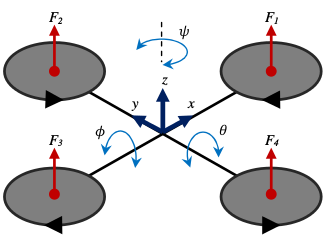
\includegraphics[width=0.5\textwidth]{./04-figuras/drone_diagram/drone_diagram_20}
    \fonte{\citeonline[p.~1]{Ariffanan2014}}
    \label{fig:drone_diagram}
\end{figure}

Os dois aspectos diferentes para se controlar sobre um quadrotor são: a sua altitude, ou seja, seu posicionamento vertical (posição sobre o eixo $z$); e a sua atitude, que é referente à devida orientação angular do \textit{drone}, ou seja, obter os devidos valores para $\theta$, $\phi$ e $\psi$. 



%\cite{Balas2007}.
%\cite{Goodwin2001}.
%\subsection{Instabilidade do Sistema}
%\label{subsec:sistemas-quadcopter-instability}
%Caracterização da instabilidade, por zeros e pólos.